% This template has been downloaded from:
% http://www.latextemplates.com
%
% Original author:
% Ted Pavlic (http://www.tedpavlic.com)
%
% Modified by:
% Charles Newey (http://assemblyco.de)
%----------------------------------------

% Declare document
\documentclass{article}

% Packages
\usepackage{fancyhdr} % Required for custom headers
\usepackage{lastpage} % Required to determine the last page for the footer
\usepackage{extramarks} % Required for headers and footers
\usepackage{graphicx} % Images
\usepackage{tabularx} % Tables
\usepackage[table]{xcolor} % Table colours
\usepackage[colorlinks]{hyperref} % For URLs
\usepackage[T1]{fontenc} % Support symbols like < and >
\usepackage{lmodern} % Format symbols properly
\usepackage{pdfpages} % Include other PDFs

% Margins
\topmargin=-0.45in
\evensidemargin=0in
\oddsidemargin=0in
\textwidth=6.5in
\textheight=9in
\headsep=0.25in
\linespread{0.97} % Line spacing

% Other setup
\pagestyle{fancy}
\renewcommand\headrulewidth{0.4pt} % Size of the header rule
\renewcommand\footrulewidth{0.4pt} % Size of the footer rule
\setlength\parindent{0pt} % Removes all indentation from paragraphs
\renewcommand{\refname}{} % Removes bibliography title

\setcounter{tocdepth}{6}
\setcounter{secnumdepth}{5} 

% Set up constants
\newcommand{\address}{
\small{
	\begin{tabular}{ l}
		Department of Computer Science, \\
		Llandinam Building, \\
		Aberystwyth University, \\
		Aberystwyth, \\
		Ceredigion, \\
		SY23 3DB \\
	\end{tabular}
	}
}

% Set up the header and footer
\lhead{\doctitle}										% Top left header
\chead{\version}										% Top center head
\rhead{\firstxmark \status}								% Top right header
\lfoot{\lastxmark \qanumber}							% Bottom left footer
\cfoot{Aberystwyth University/Computer Science}			% Bottom center footer
\rfoot{Page\ \thepage\ of\ \protect\pageref{LastPage}}	% Bottom right footer

% Set up title page
\title{
	\vspace{1.2in}
	\textmd{\textbf{\doctitle}} \\
	\vspace{0.1in}\large{\textit{\today}} \\
	\vspace{0.4in}
	{\bf{\qanumber}} \\ \vspace{0.4in}
	\version \\
	\status \\
	\vspace{0.4in}
}

\author{\authors}
\date{}


%----------------------------- UPDATE THESE FOR EACH DOCUMENT ------------------------------
\newcommand{\version}{Version: 1.0} %======================================================= DOC VERSION
\newcommand{\status}{Status: Release} %===================================================== DOC STATUS
\newcommand{\qanumber}{SE.10.FINAL.1} %===================================================== QA NUMBER
\newcommand{\doctitle}{Group 10 Final Report} %============================================= DOC TITLE

%----------------------------- UPDATE THESE FOR EACH DOCUMENT ------------------------------
%=========================================================================================== VERSION HISTORY
\newcommand{\versionhistory}{
		\begin{tabularx}{\linewidth}{| p{2cm} | p{2cm} | p{2cm} | X | }
			\hline
			\bf{Author} & \bf{Date} & \bf{Version} & \bf{Change made} \\
			\hline
			CCN & 07/11/2013 & 1.0 & Updated order of authors on cover \\
			\hline
		\end{tabularx}
}

%---------------------------- UPDATE THESE FOR EACH DOCUMENT ------------------------------
%=========================================================================================== AUTHOR LIST
\newcommand{\authors}{
	\begin{tabular}{| l | l |}
		\hline
		\bf{Contributor Name} & \bf{Role} \\
		\hline
		Daniel Clark & Project Lead \\
		\hline
		Mark Lewis & QA Manager \& Web Developer \\
		\hline
		Charles Newey & Deputy Project Lead \& Android Developer \\
		\hline
		Martin Ferris & Android Developer \\
		\hline
		Ashley Iles & Android Developer \\
		\hline
		Kenny Packer & Android Developer \\
		\hline
		Stephen McFarlane & Deputy QA \& Web Developer \\
		\hline
		Kieran Palmer & Web Developer \\
		\hline
	\end{tabular}
	% Don't edit this
	\\ \\ \\ \\ \\ \\
	\address \vline
	\hspace{0.15in} \copyright Copyright Group 10, 2014
	% Don't edit this
}

% Make title page, ToC and other introductory elements
\begin{document}
	\maketitle
	\newpage
	\tableofcontents
	\newpage

	% Begin the actual document
	%======================================================================================= DOCUMENT STARTS HERE
	\begin{section}{INTRODUCTION}
		\subsection{Purpose of this Document}
		The purpose of this document is to give both a brief overview and an in-depth report into the quality of the finished project. It is also to give a maintanence manual for both sides of the project to ensure future devlopment of the project is as simple as possible.

		\subsection{Scope}
		This document will cover a Management Summary which is a brief overview of various elements of the entire project, including it's state of completion and how the team worked to get it to its current state. It also includes a Historical Account of the Project which entails a step by step overview of the major milestones in the project in order from oldest to newest. A section for the Final State of the Project is also included which goes into more detail about exactly what parts of the software works and what doesn't. \\
		
		An individual assessment of of the performance of each Team Member is also included, to go into detail about the contribution and progress every member of the team has had over the course of the project. Lastly there is a brief critical evaluation of the team and the project which explains what we have learnt from the project and what we would change for next time. \\
		
		It will also contain a Maintenance Manual for both the Android and the Web sides of the project to ensure that the future development of the projects source code is as simple as possible. This document will also supply the management with a personal reflective report from every member of the group on how they think the experience went, plus the revised versions of the previously submitted documentation after the recommended changes have been made.

		\subsection{Objectives}
		The objectives of this document are to:
		\begin{itemize}
			\item{Give a suitable summary for submission to management to give an idea of the success of the project.}
			\item{Give an in-depth view of the projects progress for the Project Manager to use to judge the quality of the software and documents produced in the project.}
			\item{Give future developers a set of guides and materials for easy continued devlopment of all software in the project.}
			\item{Give a personal reflective report for each group member to give the Group Manager a good idea of how the project was run and how each group member felt the project went.}
			\item{Give up-to-date versions of the previously submitted versions of documents, including changes that the Project Manager and customer had suggested.}
		\end{itemize}
	\end{section}
	
	\subsection{GitHub Repository Structure}
	As a point of information, the project is stored in two repositories, so as to avoid mixing code bases (this is commonly regarded as bad Git practice) - and this also allowed us to keep our repositories under GitHub's maximum recommended size of 50mb. This also made it significantly easier to use the Android project in Android Studio with the Git integration. \\
	
	The URLs of the repositories are:
	\begin{itemize}
		\item{Document and Web Repository - \url{http://Github.com/Danyc0/CSG10.Git}}
		\item{Android Repository - \url{http://Github.com/charlienewey/CSG10.Git}}
	\end{itemize}
	
	\clearpage
	\section{End-of-Project Report}
		\subsection{Management Summary}
		The project as a whole has achieved almost everything it set out to do. The app is in full working order and is well tested with only a few minor features missing; and these can easily be added at a later date. \\
		
		One missing feature is that it is not possible to add multiple images to each Waypoint. This is because we misunderstood the specification until the last day of Integration and Testing Week, at which time we had no time to change it (this is because we thought it meant that you needed multiple photos per route, not per waypoint). The other missing feature is that the user is unable to edit Route metadata once it has been created. The website also works perfectly and has every feature specified in the requirements specification plus the added feature of a gallery at the bottom of every photo in a route. \\

		All submitted documents were submitted on time and to appropriate standards regarding the Quality Assurance standards that have been put in place. All documents were checked for errors and were checked to ensure they contained the correct material for submission. After feedback was received on the initial document versions, changes were immediately implemented ready for final submission. \\

		The main difficulties experienced during the completion of this project were illness from group members, and the adverse affects the weather had on the number of workable days for the project. Over the course of the project around half of the group have missed meetings due to illness and although all work was later caught up on, full attendance of all meetings would have ensured higher efficiency throughout the project. The impact the weather had on the projects completion has been small, but only thanks to the work done to make up for missed time by group members. \\

		As a whole the team performed fantastically, in general most team members pulled their weight and produced work of a good quality resulting in a well rounded and complete submission. A few team members throughout the course of the project did not however contribute to the submission as much as the rest of the group, which ended up resulting in them receiving a yellow card. A few other minor problems arose during the course of the project but they were dealt with quickly and didn't end up impacting the final quality of the submitted project. \\
		
		\subsection{Historical Account of the Project}
		The first thing the group did, with the assistance of our project manager, was decide on group roles - setting out who would be doing what based on their skills and experiences. We decided that Daniel would be the Group Leader because he had experience with leading a group as well as having extra time due to having only 50 credits in the first semester. The Assistant Group leader was decided to be Charlie because he was also enthusiastic about leading and was an experienced Java programmer, leading him to also be the Lead Android Developer. Stephen volunteered then to be the lead Web Developer as he enjoyed working on web design and he was doing the web modules. The rest of the group remember were then divided up into doing either Android or Web, based on where their skill set lied and which they preferred, except Mark who became the Quality Assurance (QA) manager. \\

		Next we started to decide which parts of the initial documentation submission (the Project Plan) would be delegated to who. This resulted in most of the group receiving sections of the Project Plan to complete, whilst two of the group (Mark and Martin) were told to start work on writing out the Test Specification for the next deadline. After the Project Plan submission was completed, the two who had been working on the Test Specification continued to work on that whilst the rest of the group started working on the first stages of the Design Specification. When then the results for the Project Plan submission were released Mark was given the task to making the initial changes, but only for things that could be done quickly, leaving the harder things to be changed later in the project. \\

		The Test Specification was then submitted after being Quality Assurance checked and some extra tests added after it was looked over by other members of the group. At this point the Design Specification was coming along nicely and now the two who were focussed on the Test Specification now joined the rest of the group in working different sections of the Design Specification. \\

		After a few group meetings involving making some of the larger design decisions we eventually had a Design Specification that was ready for submission and so after being QA checked, it was submitted on time. This meant that everybody could now start coding and working towards a working prototype for the Prototype Demo. Stephen and Kieran were set to work together on making a statically generated version of the website to demonstrate what it would look like, whilst the rest of the group were given individual parts of the Android App to focus on and get working, e.g. Daniel was to work on getting Post Requests to his server working using JSON, Charlie was to allow the taking of photos, etc. The plan was then to merge all the working parts of the App together. \\

		When the time came for the Prototype to happen Stephen had finished the static website on his own, with minimal help from Kieran and most sections of the Android app were complete but the parts had not been merged together. The demonstration went well with the 'customer' commenting that no other group had got HTTP Posting working other than us at that stage. It was at this stage that it was decided to give Kieran his Yellow Card as up until this point he had not contributed anywhere near as much as others in the group. \\

		After that we got the feedback on the Design Specification and Mark started work on making the changes needed whilst the rest of the group started on the finished products for both web and Android. After Mark had made the initial changes it was at this point that he volunteered to be in charge of the database interaction side of the web system, as using SQL and doing database work was relatively easy for him. This was also because he had noticed that the web side had not been progressing at the same rate as the Android development. Over the Christmas holidays not much work happened on the web side - some slight UI changes and not much else, whereas on the Android side each element demonstrated in the prototype had finally been merged into one united app. \\

		At the start of Integration and Testing week the Android app seemed very close to completion but the Web was still lagging behind, with still no facility for receiving HTTP POST requests. Throughout ITW Charlie, Martin and Daniel were focussing on adding features and fixing bugs in the Android code whereas Ashley was working on the User Interface and Kenny was doing continuous testing on any new features to check for any bugs that got introduced during development. On the web side Stephen was working on getting the Website to be generated using data from the Database (with some help from Charlie at the end) whilst Mark worked on developing the Database and adding data to it from the HTTP Posts. Kieran was also given the task of redesigning the web interface and updating the docs, specifically the Test Specification so that we were clear which tests we passed and which tests we still needed to work on passing. \\

		After ITW the entire group was working on documentation, most of the group was making the recommended changes to the previously submitted Docs whilst Daniel wrote the End of Project Report and Charlie compiled each section into one LaTeX document, doing Quality Assurance checking as he went. We realised at this point that a lot of the previous changes Kieran had made to the documentation were sub-satisfactory and therefore it was decided not to revoke his Yellow Card.

		\newpage
		\subsection{Final State of the Project}
		Both sides of the delivered software package work almost perfectly to meet the delivered specifications as set out in the project documentation. 
		The app contains functionality to create a walking tour containing the title, short description and long description for the route, as well as a title, description and photo for as many waypoints as the end user wants to create. The only point at which this strays from the set specification is we have not yet implemented the limit to restrict only single word titles for each walk. \\
		
		The GPS coordinate for the tour are started gathering from the point at which the user finishes entering the general route details, then an extra set of coordinates are attached to each waypoint created as part of the tour along with its Unix Epoch timestamp. When it comes to adding photos to the created waypoints, the user is prompted whether they want to take a photo from their camera or add a photo which is stored in their phones gallery as per the specification, however due to an initial misunderstanding of the documentation only one photo is able to be added to each waypoint. \\
		
		The route is able to be cancelled at any time by pushing the 'back' button on their phone, which will then prompt them to whether or not they truly wish to cancel recording the route. Data sent to the server after final completion of each route is sent via an HTTP POST request containing a set of JSON key-value pairs with a MIME-Type of "application/json", the JSON format was chosen over the MIME format because the existing libraries for Android and PHP made the specifics of coding the POST request far simpler as well as JSON having the extra benefit of being more human readable than just standard MIME. We informed the customer (Bernie Tiddeman) of this change during the design phase of development and he accepted the change. \\
		
		When the user decides to switch android applications the app will cache the stored data and reload it when the user restarts the app. This process will also handle when the users exits the app for long periods of time and the Android OS kills the App to save RAM. A bug we found in this part of the feature through testing though is that the list of data is not refreshed until you add a new waypoint, however the data IS there either way and can be sent to the server. The apps service will also continue to run in the background recording the GPS track even if the app does not have focus, meaning the user can continue to use the phone for other things whilst walking between waypoints and then restart the app when they decide to make a new waypoint. \\
		
		On the web side of the software package the user is able to pick any uploaded route from the drop down box and all the information about that route will be displayed to the user, the details of the route itself are displayed at the top of the page, whilst the details of each waypoint are stored within markers on an interactive map in the centre of the page. \\
		
		Once data has been successfully received by the web server it will return a standard HTTP 200 code confirming that it received the data, or another code depending on what problem was encountered in the transmission. This will then be checked on the android app and an appropriate message will be displayed to the user regarding the success of the delivery, and if successful, they will be given the opportunity to start a new route.

	\clearpage
		\subsection{Performance of each team member}
		\subsubsection{Daniel Clark - Group Leader}
		As a whole the duties taken on by the group leader were the organisation of the project, delegation of tasks, making sure that the team were happy and comfortable with their assigned work as well as ensuring that the project was progressing at the desired rate. \\
		
		The group leader's attendance to all whole group meetings was ensured, however some group meetings only required attendance by each side of the programming team and thus the group leader did not always attend. Throughout Integration and Testing Week the group leader was present every day from 9-6 and made sure to supervise any problems the group was having and dealt with any problems involving members of the group that were not arriving on time. Throughout the project the group leader has also input significant amounts of functional code into the Android development, as well as taking a large role in debugging and solving problems found by other members of the team on both the Android and PHP sides of development. \\
		
		Throughout the project a significant degree of enthusiasm for the project has been maintained, however, post-Integration and Testing Week enthusiasm for the project started to lower as the deadline approached. In general work produced by the group leader was to the standard expected by the rest of the group and all duties were taken care of appropriately. That said, the efforts of the Assistant Group Leader (Charlie Newey) to keep the project on course has compensated for some organisational shortfalls of the project leader throughout the later half of the project. \\
		
		{\bf Acceptance:} I (the group leader) as writer of this document, agree with the above self-appraisal.


		\subsubsection{Charlie Newey - Assistant Group Leader and Lead Android Developer}
		The duties taken on by Charlie extend far further than the limits set out by his official project roles. Officially his role entails a lot of the group leaders responsibilities but to a lesser degree, as well as taking charge of the Android development and making sure that everyone within the Android coding team knew exactly what needed doing and which tasks they were assigned to. On top of maintaining a high quality of work in his official roles he also continued to support the group leader and compensate for any shortcomings he came across throughout the project. On top of the tasks he was assigned he has also made contributions to the Quality Assurance of both the documents and all parts of the code and spent a not-insignificant amount of time working with the team's Web developers to fix bugs and add features to that side of the project in any free time he had during Integration and Testing Week. \\
		
		Charlie made attendance to almost every meeting of both the general group and the Android development meetings although he did sometimes turn up late. During Integration and Testing Week he consistently arrived an hour after the start to the day, but he always made up for this by spending extra hours in the evening working on the project. Charlie took one day at home during the week (but continued to do work) as he was expecting a large delivery - this was out of his hands as it had originally been organised to not clash with ITW, but the adverse affects of the weather delayed ITW by a week, thus causing the problem. \\
		
		Charlie's enthusiasm for the project has been high all throughout the project often spending extra hours perfecting sections of work he and others had produced. His high enthusiasm seems to be driven by the desire for the entire group to receive over 70\% for the project and he went out of his way to try and achieve this. The quality of work produced by Charlie throughout the project has been strong, producing readable and complete sections for documentation when required, and producing a high quality of well documented code during Integration and Testing Week. \\
		
		{\bf Acceptance:} I, Charlie, agree with the above statements. I made a large effort to restore any project time lost, and did so several times over. I feel, however, that my contribution to the the project was a little higher than my 'fair share', and that I had to pick up slack left by some team members. With that said, I would do so again if it ensured the project reached successful completion. The comments on my attendance during ITW are fair, but reflect the extremely late nights I was working on the project - long after the day had officially ended.


		\subsubsection{Stephen Mcfarlane - Lead Web Developer}
		Stephen, as he had experience of PHP, was set the duties of writing the majority of the projects web side. He alone produced a working static version of the website for the prototype submission and during Integration and Testing Week adapted it to work with dynamic data pulled out of the database. Stephen made it to all scheduled meetings before and after Integration and Testing Week, however during the early part of ITW he was at least 2 hours late on most days. Despite being late on some days during ITW, he always made the effort to make up work he'd missed during the evening so that his tasks were completed and up to date before the next morning, meaning that the project was not held back. When it comes to Stephen's attitude towards the project, he has continuously proven to be a consistent hard worker, every task set to him was completed on time and it was obvious to see the progress he was making as time progressed. \\
		
		The code produced by Stephen for dynamically delivering the website to the user was completed to a good quality, however the JavaScript which was used in conjunction with the Google Maps API to display the route to the user could have been written in a tidier and more readable way. Towards the end of ITW Stephen was struggling with getting the last part of the website working, but after a code refactor and some help from Charlie, a solution was found. The parts of the documentation he wrote to go along with the project were complete and well written to a good standard. In general Stephen is very easy to work with and will always complete whatever he is given to the best of his ability. \\
		
	{\bf Acceptance:} I, Stephen, have read this and approve this report.


		\subsubsection{Mark Lewis - QA Manager and Web Developer}
		Mark's original role was solely to be the QA Manager, a job that during the pre-Integration and Testing Week stages he did to a good standard - making sure that documents were completed to the correct standard before submission. When the group started working on getting the final code working however, Mark offered to lend a hand with the Web Development as he had some experience with working with SQL and the database technology. \\
		
		Mark made it to almost every meeting and took up the general role of writing the meeting minutes. If he was ever unable to attend, he notified me beforehand and work was set remotely. During ITW Mark was often the first to arrive just before 9am and stayed until the end of the day. When Mark realised that he could use his skills to benefit the group by working alongside the other Web Developers and volunteering himself for the extra role it was obvious that he was motivated to make sure the project was a success and was completed on time. \\
		
		In his role as QA manager Mark also spent time at the end of Integration and Testing Week improving the quality of the back-end web code to ensure it met the coding standards that had be set out. Over every aspect of the project that Mark worked on he made sure to produce a quality piece of work. Even from the start, the minutes of each meeting were taken professionally without prior instruction, documents were QA checked before submission on time and his code was well written and well commented despite needing some occasional help from other group members. \\
		
{\bf Acceptance:} Mark agrees with Dan's comments. 


		\subsubsection{Martin Ferris - Android Developer}
		Martin's role as an Android Developer throughout the project has led to him producing a significant amount of the code for the Android App, as well as spending time at the end of the project finalising the document changes. Throughout the project Martin's attendance has been fantastic, he turned up to virtually every organised group meeting and made it to every day of Integration and Testing Week. The only problem in Martin's attendance was that he very rarely showed up on time for ITW, however that did get better as the week went on and he always made up for missed time in the evenings. \\
		
		He has had a high level of enthusiasm throughout the project consistently finishing work and asking what needs to be done to improve the final product. Martin took the responsibility of writing the sets of JavaDoc comments for almost all of the Android code and got it ready for generating the final HTML JavaDoc. He also did work on building the UI for some of the screens working with Android Studio and directly with the XML. He is often willing to go the extra mile in ensuring documents are completed on time for a deadline and that feedback from the customer is appropriately dealt with. \\
		
		The quality of work the Martin produces is consistently of an acceptable standard in both code and documentation. Although at times he struggled in fixing bugs and implementation problems in the code, but with minimal guidance he eventually worked through every problem. Generally Martin is very easy to work with and, with the right support, will produce quality solutions to problems. \\
		
{\bf Acceptance:} I, Martin, have read this report and approve of Daniel's comments.


		\subsubsection{Ashley Iles - Android Developer}
		The role set out for Ashley initially was to be one of the Android Developers and out of everyone he stuck to his role the most.
		
		His attendance through all of the official meetings was generally very good, however he missed some of the non-official meetings. This was never due to him being unenthusiastic, it was because the meetings were always organised via Facebook and Ashley has never been a strong Facebook user. Ashley's attendance during Integration and Testing week was not fantastic, often turning up late and on one day he didn't turn up at all, but that was due to illness (although we were only told this the day after). Despite this however he did partially make up for that by staying late one one night to make some final changes. \\
		
		Pre-ITW Ashley did work on the designs for the User Interface of the Android app including the initial designs and the initial way the user would use the App in the Sequence Diagram. During Integration and Testing Week Ashley ended up mainly focussing on the User Interface design for the Android App, as he generally has a good eye for what looks good. This involved things like working with the UI tool in Android Studio as well as directly editing the XML when he needed to. It also involved a reasonable amount of editing images that Charlie had taken previously for use as the backgrounds for the App. He also did work with the timestamps in each waypoint and was generally considered the go-to guy whenever the XML was involved. \\
		
		Ashley's quality of work was generally good, however at times it required quite a lot of effort to get work out of him in the first place. \\
		
{\bf Acceptance:} I, Ashley Iles, do agree that the above is an accurate description of my involvement in this group project.


		\subsubsection{Kenny Packer - Android Developer}

		Kenny was assigned to be part of the Android Development team. Throughout the project Kenny spent most of his time working on developing the Android app as well as writing the initial versions of some of the documentation and making the changes as recommended by the customer. \\
		
		Due to timetabling commitments it has meant that he has had to miss some of the meetings planned with short notice, but he is always happy to meet after the meeting to discuss what needs doing. During Integration and Testing Week Kenny showed up every day and continued to work on the App with the rest of the group, he also took the lead in testing the app after each new feature was marked as complete, often flagging up major bugs which needed fixing. Kenny also headed up making the more detailed visual design decisions for the app, e.g. designing the apps logo. \\
		
		Throughout the project Kenny would always be up for taking on any task set and was not afraid to ask for help when he needed it. He often seemed to feel more comfortable working in tandem with someone else on a task rather than working completely on his own. He also was often used as a method of coordinating with Kieran when he was not available by other means or in meetings. \\
		
		The quality of Kenny's work stayed consistent all the way through the project, always completing documentation as needed which generally only needed minor spelling and grammar checking. Although Kenny did not contribute a significant amount of code, the code he did produce was of high quality. \\
		
{\bf Acceptance:} Pretty much true, no issues with this evaluation - Kenny


		\subsubsection{Kieran Palmer - Web Developer}
		Kieran's role in the project was set out as a Web Developer, whose role was mainly to support and contribute to the web front-end side of the project. He also took charge of making the initial changes to documents once they were returned after the first submission. Throughout the project Kieran has missed a significant amount of group meetings - both official timetabled meetings and individual group meetings. Kieran also missed a few days of Integration and Testing Week and on the days he did attend, was often late. \\
		In the first part of the project Kieran mainly focussed on documentation of the web side, producing parts of the document like the web side Sequence Diagram. During Integration and Testing Week Kieran's main focus for the project was on improving the UI for the web design. At the start of the project it seemed that despite his initial enthusiasm, the progress made by Stephen left Kieran without the opportunity to contribute at that stage of the project. Kieran's general attitude towards the project has been reasonably good whilst in meetings, however between meetings his contributions to the project seemed to dwindle. Towards the end of the project Kieran's attitude seemed to improve, often asking what extra work he can do an what he could contribute to. \\
		
		The quality of documentation produced was generally good with normally only minor corrections needed.	Kieran has struggled throughout the project on learning to use the Git version control, always needing supervision from other team members before committing any progress he makes. \\
		
		I think with more managed time and meetings Kieran could be a much more valued member of the team. \\
		
{\bf Acceptance:} I, Kieran, agree with what Daniel has written about my efforts in the group project. I acknowledge that my contributions were poor and I appreciate the help given to me by other members of the team.


		\subsubsection{Critical evaluation of the team and the project}
		As a whole, the team performed fantastically, which resulted with a finished product I think we can all be proud of producing. The contributions of some team members significantly outweighed the contribution of others, which led to an unbalanced separation of the work. However on average the team pulled together and balanced out all the work that needed doing. \\

		I think the project as a whole could have been improved by spending more time focussing on making sure the Git version control was nailed down and fully understood in everyone's mind, because it allows for far greater collaboration even when group members aren't in the same room. Another improvement I'd make if I did this again would have a better adopted communications system due to the fact that neither Kieran nor Ashley spend much time on Facebook, meaning they missed out on a lot of the communications that were happening. \\

		As a group, we all agree that the most important lesson learned about working on software projects is that communication is key, everybody needs to know exactly what's happening, when it's happening and what they're meant to be doing. Another important lesson is about making sure that the less able people involved in a project feel like they are making a worthwhile contribution to the project to make sure that their enthusiasm stays high and they produce work to the best of their ability. Something else we've learned that will help us in future group projects is the value of having dummy systems when working on two platforms, e.g. we had a dummy web server running that we used to test that the Android app could send data long before the actual web server was functional. Furthermore, the way we structured this project is proof to us that good planning, good testing and incremental development really do help to produce a quality product at the end.
	
	\begin{section}{APPENDICES}
		Over the next few pages, various appendix items are included:
		
		\begin{itemize}
			\item{Reflective reports from all team members.}
			\item{A test log - which should provide sufficient evidence of testing and the functioning state of the application.}
			\item{Revised and updated versions of the Project Plan and Design Specification}
			\item{A full maintenance manual to aid any future software engineers in solving problems and improving the project}
		\end{itemize}

		This should hopefully give a full overview of the project's structure and measured success.
		
		\vspace{3in}
		\begin{center}
			This space is intentionally blank
		\end{center}
		
		\clearpage
		\subsection{Reflective Reports}
			\subsubsection{Daniel Clark}
				\begin{tt}
				Daniel's Personal Reflective Report \\
				=================================== \\

				I think on balance the project went extremely well. As with other groups it took us some time to get to know each other and learn each others strengths and weaknesses, but as time progressed the speed and efficiency at which we worked greatly increased. One of the major problems we had in the group to start was that, having never worked together before, we had no idea what each other considered as 'good', and what we all expected of each other. As the project progressed it was obvious that some group members were more motivated to succeed than others, but in general there was definitely a positive attitude toward the group throughout. During Integration and Testing week the group really started to become a unit, where everybody knew what they were doing and always knew what the next step to take was. \\

				As an individual I really enjoyed the project, learning how to use development tools and techniques effectively, learning about the Android development environment and how powerful the Android API is. Also learning about PHP, as language I've never even touched before, was extremely interesting and has given me a much better background in the topic for further progression. \\
				As Group leader I feel that I did a good job leading the team, maybe at times not the best but I still think I've managed to lead the team into getting the desired result. Leading a team with such varied abilities has taught me an awful lot about how important good communication is, and how it's important to make sure that each member of the team feels like they are making a valuable contribution to the project. I also learnt that being liked by your group is extremely important in keeping up group moral throughout long projects, as without that the entire group ethos can fall down. \\

				Although I did end up spending massive amounts of time on the project, I always expected this and that is one of the reasons I put myself forward as group leader. This is because I was only taking 50 credits in the first semester which left me much more time to focus on the project and its development. \\

				If I were to ever repeat the project or one of a similar nature, I'd have made sure I put more effort into making sure every team member got the support they needed and felt that they could ask for extra help/resources if needed. Also, although I tried to enforce good Git practice right from the get-go, next time I would definitely focus more on making sure every single team member was completely happy with using it's basic operations and how to deal with conflicts. \\

				Total time spent on project \\
				--------------------------- \\
				Estimated project work time 130-140 hours. \\
				\end{tt}
		
		\clearpage	
		\subsubsection{Charles Newey}
		\begin{verbatim}
		Personal Reflective Report
		==========================

		Overall, I'd feel the project was successful. Despite being slow to start, the group
		began to work more effectively as a team during Integration and Testing Week, to a point
		that our "turnaround time" for bug fixes was less than an hour. The majority of the app
		functionality was implemented and the vast majority of tests passed.

		The major difficulty of the project was the process of getting to know the team's
		abilities initially, it was difficult learning everybody's strengths and weaknesses.
		We worked together as a whole, although I feel perhaps that I did more work than
		was my 'fair share'. This was due to perhaps underestimating the amount of work that
		would be involved in the project, and the learning curve for the project tools 
		(Git, GitHub, and LaTeX) all presented a challenge for the team and was a recurring
		difficulty throughout the project, requiring help from myself and Daniel.

		We also faced a number of problems with group members, including late submissions of
		work from some group members (for internal deliverables), poor attendance, and extremely
		poor communication. This led to a number of complications that I feel myself and
		Daniel have had to take on disproportionate workloads to compensate for.
		In all, I did a very large portion of the overall work, and this has been a
		major frustration to me during the course of the project.

		Despite this, I enjoyed the project. The Android development was interesting,
		as well as complementing my own skill set as a developer. Working on a code base
		with a small team was a new experience for me - one that I enjoyed overall. Working in
		a team enabled better discovery of flaws, faster turnaround time on bug fixes, and
		more efficient code as we held informal code reviews often during Integration and
		Testing Week. Outside of ITW, the team were generally good to work with, although
		the difficulties mentioned above did somewhat sour the experience.

		If I were to repeat the project - personally, I'd have learned a little more about 
		Git and GitHub before the project started. Learning about Git is one thing, but it's
		very different to use in a group setting, and can be quite a steep learning curve for 
		a new user. This became less of a problem as the project progressed, and I was able
		to help others - but this was initially a problem as it would have been more useful 
		to be able to help some of the other team members with learning project tools - 
		instead of spending time learning them myself.

		Total time spent on project
		---------------------------
		Estimated at 135 hours. (Summary of time in blogs + 10 hours for final document)
		\end{verbatim}
		
		\clearpage
		\subsubsection{Stephen McFarlane}
		
		\begin{verbatim}
		Personal reflective report
		==========================
		
		Well I think the group project went great the group worked well as part of
		a team and we got the project working on both web and app side. I learnt a decent
		amount about how to use google maps when creating a web page which means
		I learnt more javascript, also with the database interaction I had to do
		some PHP, SQL and XML. The only thing I would have changed was learning how
		to use Git before the project started as it was difficult to learn while 
		doing and made some minor errors.

		We had a few problems with the website like not having a database up and 
		running for a while and the database interaction with the Google maps JavaScript, 
		but this was all sorted out and was finally fixed.

		Personaly I found the project enjoyable I learnt alot and was fun at some times. 

		total amount of hours on project :  60-65 hours over pieces of work and 30 
		hours looking up information to create website such as researching Google 
		maps and php techniques to get the website to work.

		Total hours : 90-95
		\end{verbatim}
		
		\clearpage
		\subsubsection{Mark Lewis}
		\begin{verbatim}
		Mark Lewis - 31/01/14
		====================
		Role: QA Manager/Web developer

		Review
		------
		I think that the project went very well. The start of the term involved alot 
		of documentation which we completed and got good grades on. Then when it came 
		to producing the system I felt it went better then I expected it to go. I was 
		mainly involved with the web side of the system, there were a few problems 
		which we encountered and at the beginning I didn't expect everything to go 
		smoothly. But these were all fixed and all the requirements where met.
		
		Overall I probably spent between 90-100 hours on the project.
		\end{verbatim}
		
		\clearpage
		\subsubsection{Martin Ferris}
		\begin{verbatim}
		Martin Ferris - 31/01/14 
		=======================
		Role: Android Developer

		Personal Reflective Report
		--------------------------
		Overall, I think the project went well. There was really good communication throughout
		amongst the group, and I feel that we produced a final product to a high standard.
		At the beginning of the project I was a bit nervous about being a developer, but everyone
		was supportive and I never faced a problem that I could not solve even if it did take 
		some time to get through.

		I really enjoyed learning how to develop android programs. It was challenging but 
		rewarding when we succeeded and reached our goals. I feel we had the right 
		approach by having lots of short term goals, opposed to trying to complete a whole 
		segment of the program in one go.

		If I were to repeat the project I would have liked to have been taught Git 
		in a more practical way, but thankfully my group members had some Git 
		experience. Also, I would have used the advisory service more as I wasted 
		a lot of time on bugs.

		Total time spent on project
		---------------------------
		Estimated at 120 hours.
		\end{verbatim}
		
		\clearpage
		\subsubsection{Ashley Iles}
		\begin{verbatim}
		Ashley Iles: Android Dev Team
		==========
		Overall I do belive that the group that I was part of was quite sucessful,
		the final product are two very functional and easy to use pices of software.
		My previous, but limited, experience / knowledge of Git and Github was very
		useful during the project. This resulted in myself requiring help with Git
		to be a very infrequent event. When refining the UI desing in android studio
		that either the other group members or myself had created I found myself
		frequently editing the XML files directly. Cleaning up the mess and unnecessary
		attributes that the IDE had created and left behind was quite satisfying.
		
		That said I found myself feeling underwhelmed and rather unmotivated, 
		especially compared to others in my group. This feeling did change during 
		the testing week, working in close proximity to my other group members was 
		something I found very beneficial.

		Estimated time spent on project ~70 hours.

		\end{verbatim}
		
		\clearpage
		\subsubsection{Kenny Packer}
		\begin{verbatim}
		Kenny Packer - 31.01.2014
		===============
		Role: Android Dev Team

		Its done, more or less, its done. And it works really well.

		I'm glad the app works really well. I'm also glad that I learnt some 
		new things, like being able to use GitHub (sort of). I also got to create the
		 mascot/icon for our app, write some code, field test the app, point out errors,
		and just generally being useful to my group. I'm not the strongest programmer, 
		or computer science student in general, so I felt I had to be useful wherever 
		I could to compensate for this. The fact that we had a really good leader 
		and deputy, meant that I could easily ask for help with any project stuff, 
		and that meant I could get a good amount of work done. I improved with 
		computer science stuff, which is good. The fact that we managed to 
		create something useful (in theory), from basically nothing but an 
		IDE and some programming know how. In a general sense, Its renewed 
		my faith in programming in Java. 
		
		Total time spent on project
		---------------------------
		40+ hours
		\end{verbatim}
		
		\clearpage
		\subsubsection{Kieran Palmer}
		\begin{verbatim}
		Personal Reflective Report

		I feel that the project was overall enjoyable and I learned a considerable
		amount. However I do feel that I did not apply or commit myself as much 
		as I could, but realising that is positive. I have gained experience from
		this project and I have grown academically and personally. The main aspect 
		that I appreciate that it was a productive break from learning and being 
		able to apply what I have already learned was refreshing.

		There were issues during construction of the software but over coming 
		them in teams was very helpful in gaining usable experience.
		
		Total time spent on project
		---------------------------
		Estimated at 40 hours
		\end{verbatim}
		
		% Include Maintenance Manual
		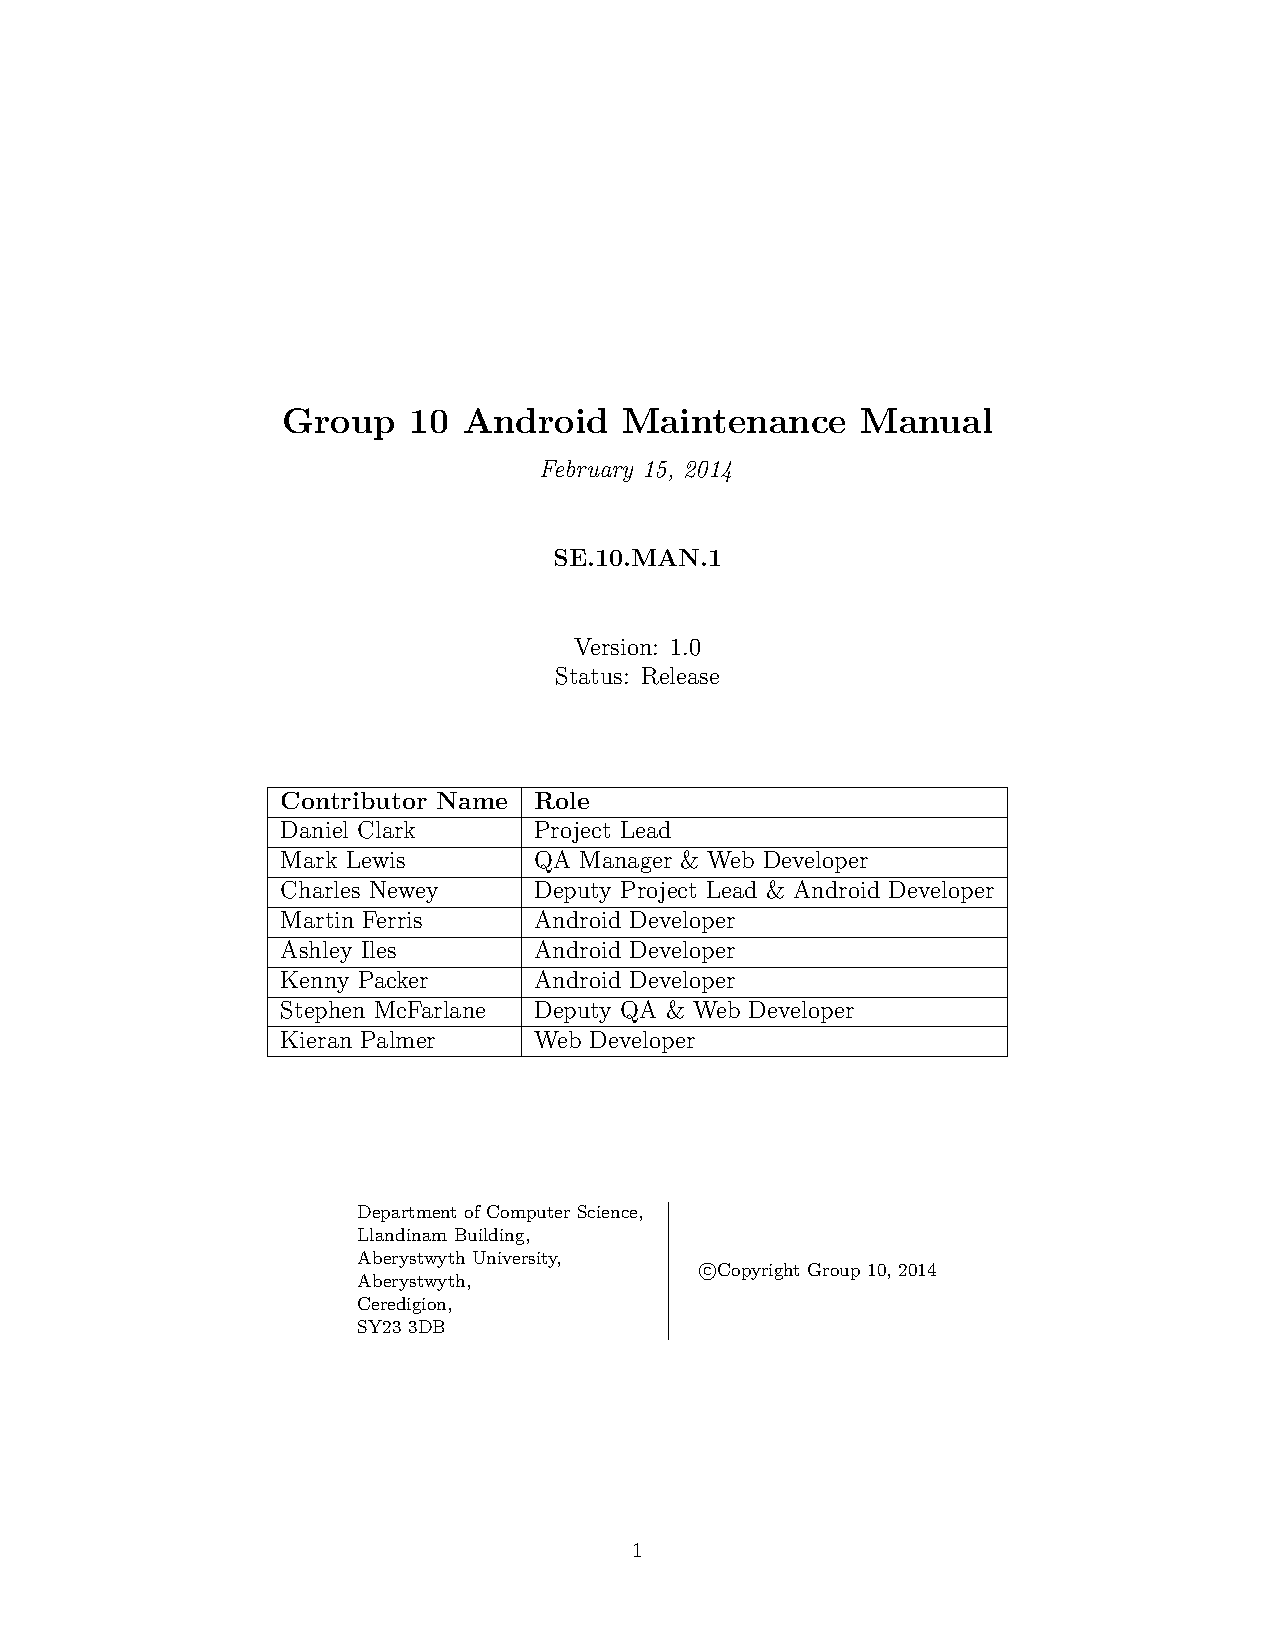
\includepdf[pages={-},addtotoc={1,subsection,2,Maintenance Manual,Maintenance Manual}]{docs/Maintenance_Manual.pdf}
		
		% Include test spec and test log
		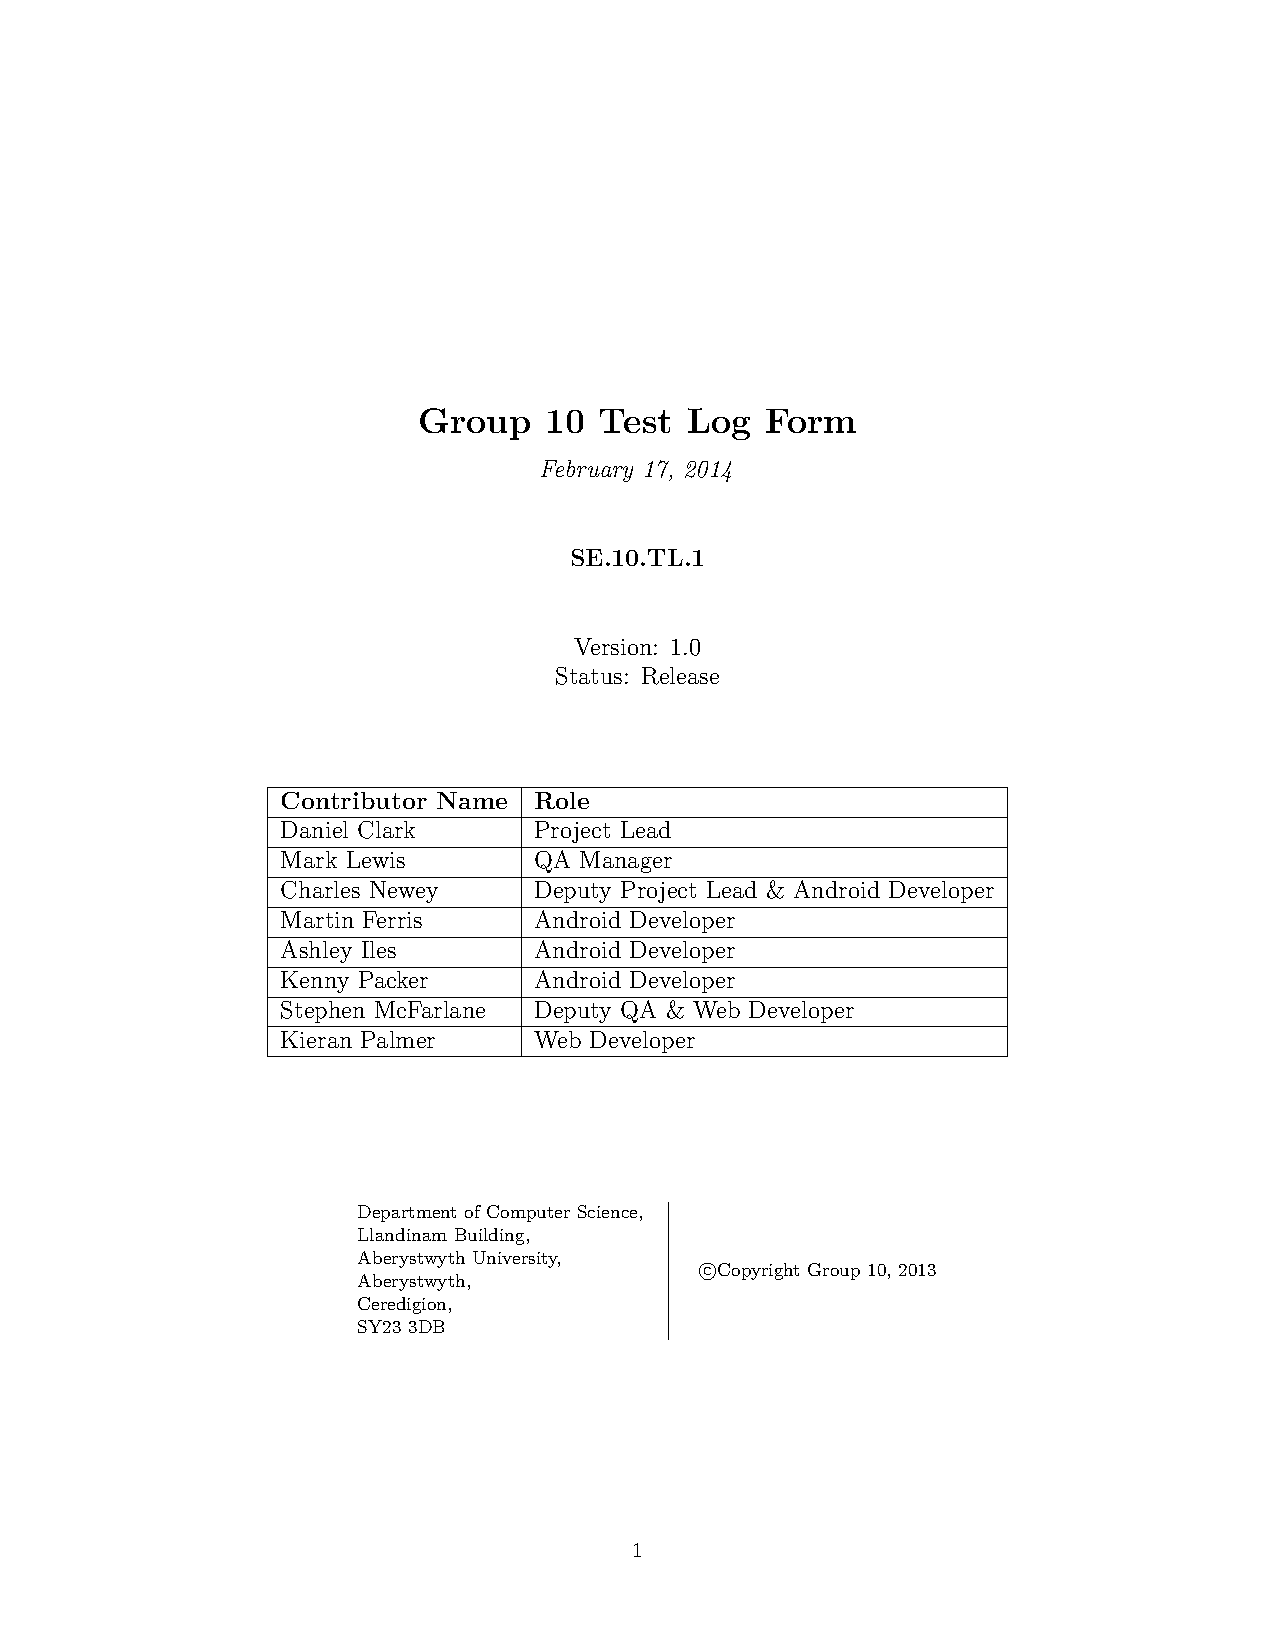
\includepdf[pages={-},addtotoc={1,subsection,2,Test Log,Test Log}]{docs/Test_Log.pdf}
		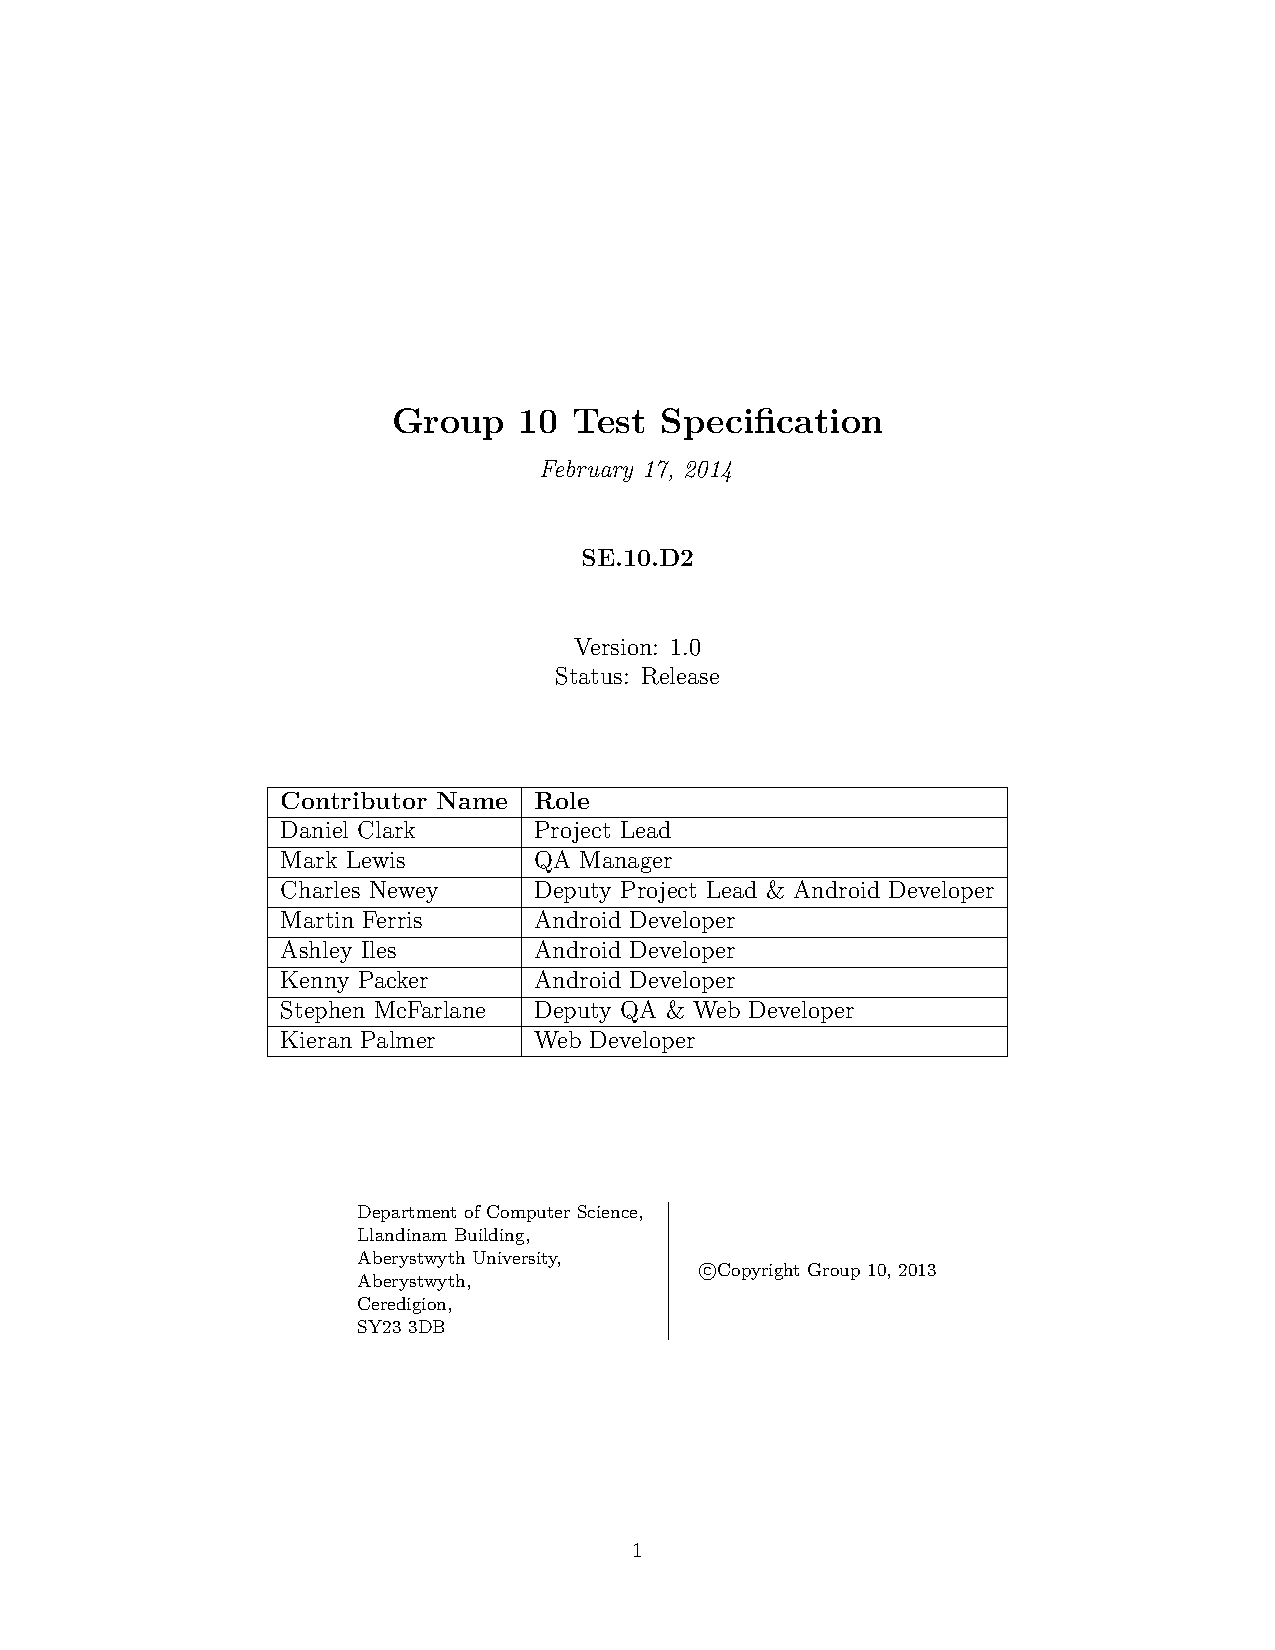
\includepdf[pages={-},addtotoc={1,subsection,2,Revised Test Specification,Revised Test Specification}]{docs/Test_Spec.pdf}
	
		% Include revised original docs	
		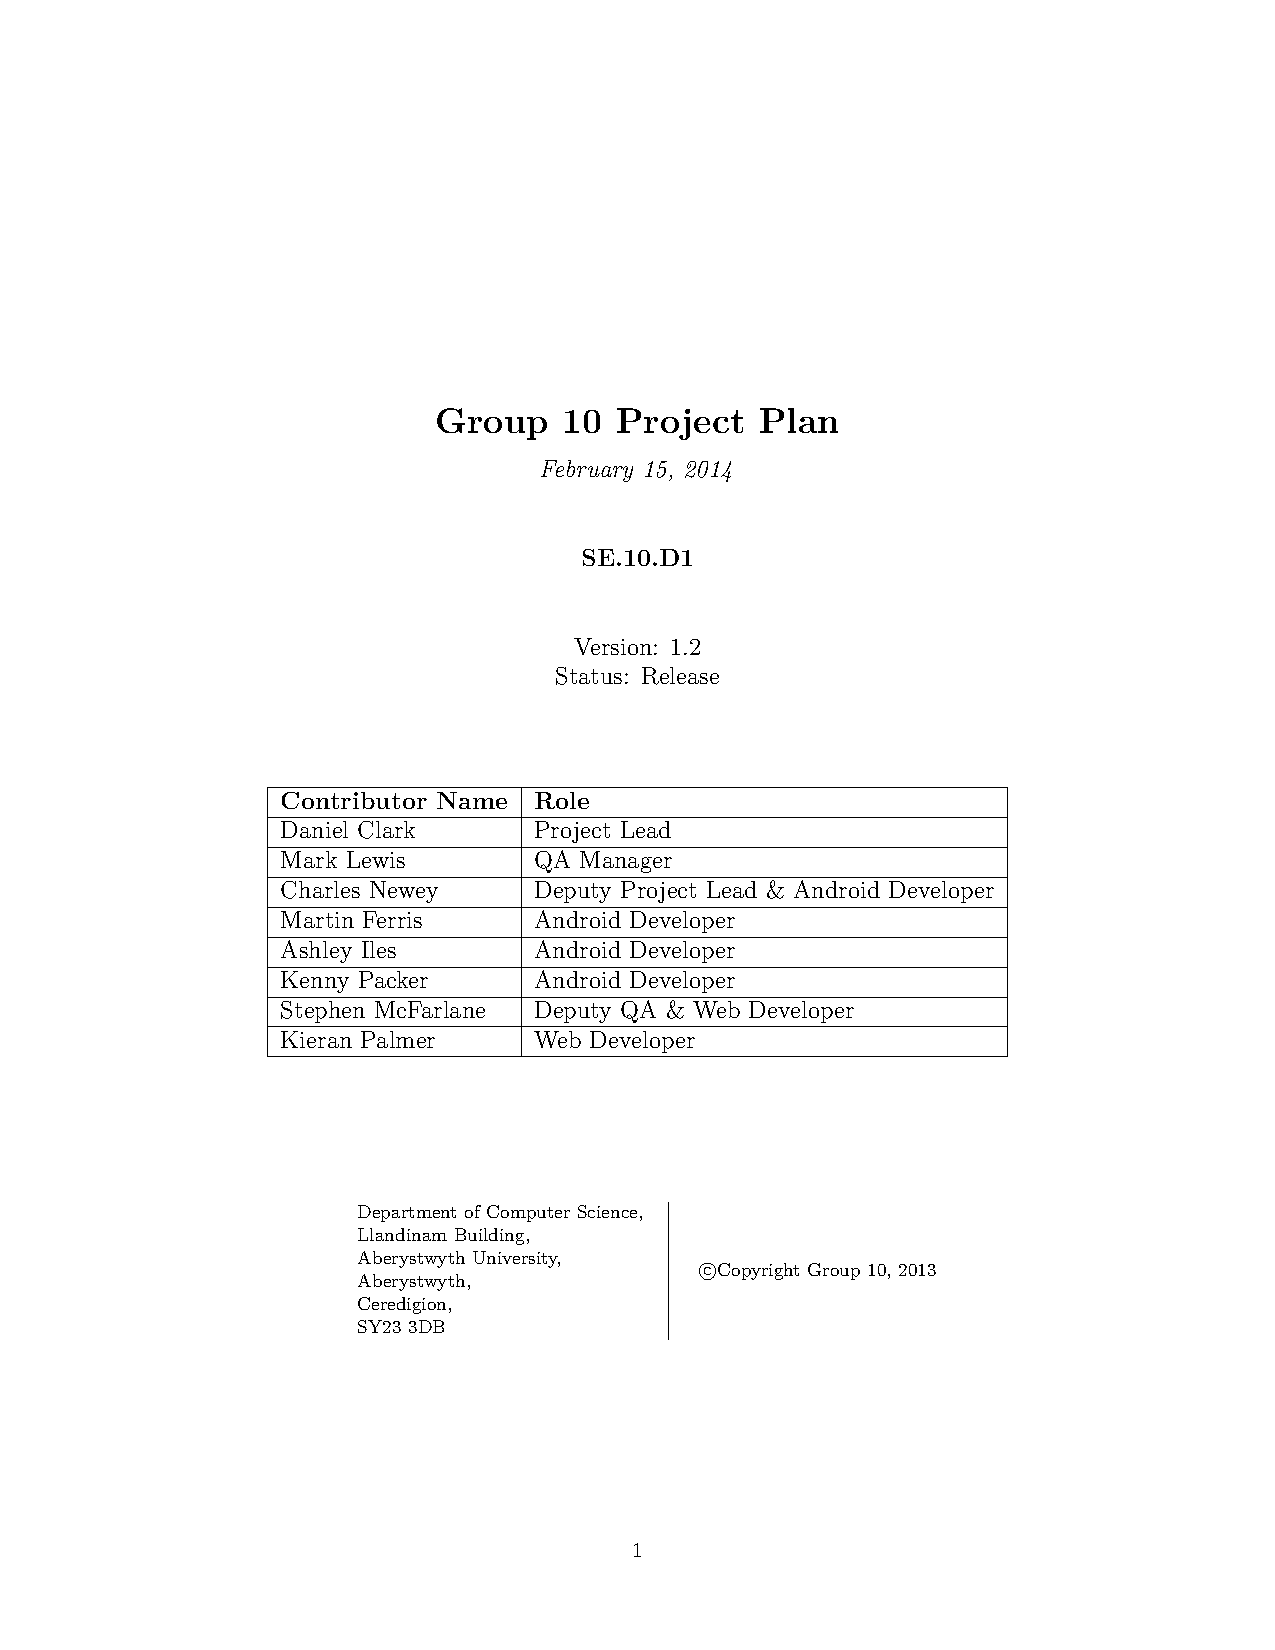
\includepdf[pages={-},addtotoc={1,subsection,2,Revised Project Plan,Revised Project Plan}]{docs/Project_Plan.pdf}
		
		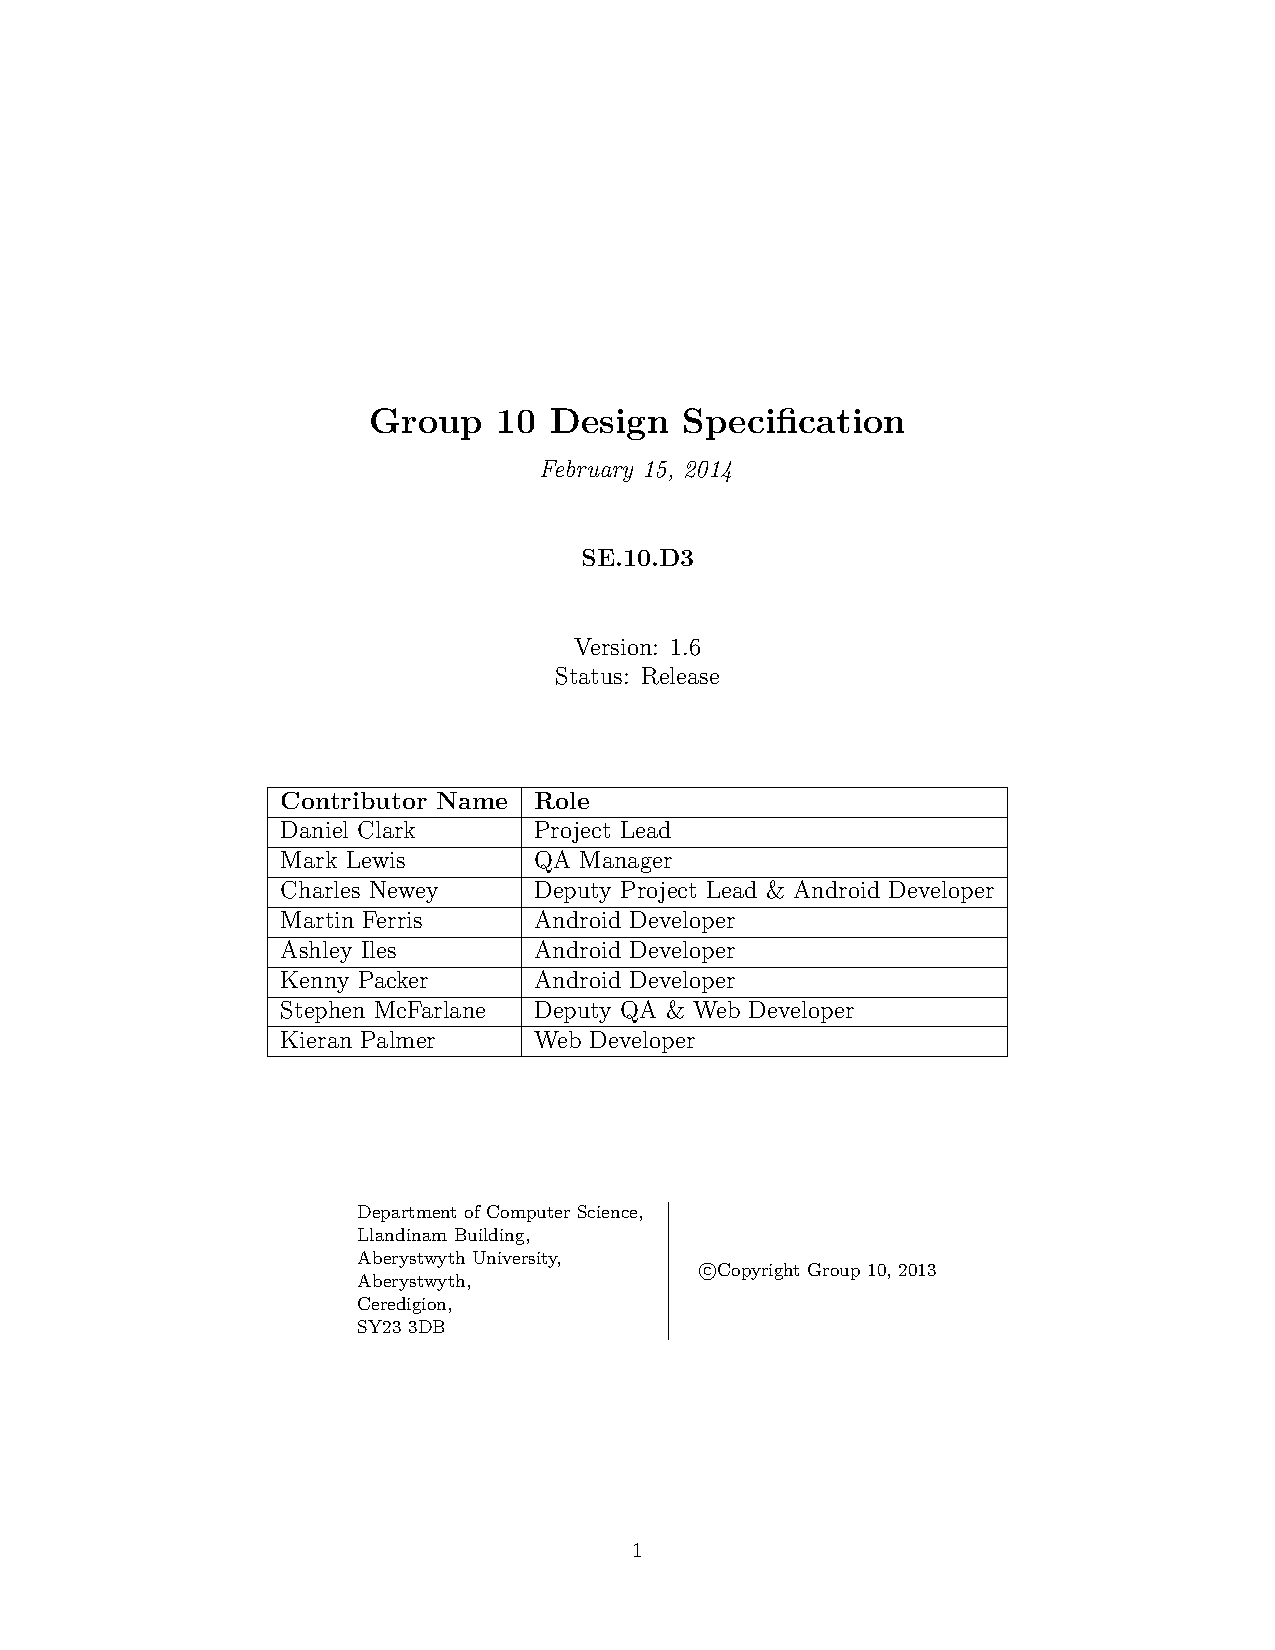
\includepdf[pages={-},addtotoc={1,subsection,2,Revised Design Specification,Revised Design Specification}]{docs/Design_Spec.pdf}
	\end{section}

	% Include references here (edit the References.bib file)
	\nocite{LaTeXTemplate} % DO NOT EDIT

	% Format bibliography/refs
	\newpage
	\begin{section}{REFERENCES}
		\bibliographystyle{acm}
		\bibliography{References}
	\end{section}
	
	\vspace{1cm}
	\begin{section}{VERSION HISTORY}
		\versionhistory
	\end{section}
\end{document}

%									Useful bits and pieces
%\begin{section}{section_name}								% Start section
%\end{section}												% End section
%\begin{center} \end{center}								% Center stuff
%\includegraphics[width=0.75\columnwidth]{example_figure}	% Insert image
%\pseudocode{filename}{caption}								% Insert highlighted code snippet
%\clearpage													% Clear page after section
%\url{http://www.google.com/} 								% Include URL
%\nocite{citationName}										% Cite to bibliography (but not to text)
%\cite{citationName}										% Include reference
